%%%%%%%%%%%%%%%%%%%%%%%%%%%%%%%%%%%%%%%%%
% Short Sectioned Assignment
% LaTeX Template
% Version 1.0 (5/5/12)
%
% This template has been downloaded from:
% http://www.LaTeXTemplates.com
%
% Original author:
% Frits Wenneker (http://www.howtotex.com)
%
% License:
% CC BY-NC-SA 3.0 (http://creativecommons.org/licenses/by-nc-sa/3.0/)
%
%%%%%%%%%%%%%%%%%%%%%%%%%%%%%%%%%%%%%%%%%

%----------------------------------------------------------------------------------------
%   PACKAGES AND OTHER DOCUMENT CONFIGURATIONS
%----------------------------------------------------------------------------------------

\documentclass[paper=a4, fontsize=11pt]{scrartcl} % A4 paper and 11pt font size

\usepackage[T1]{fontenc} % Use 8-bit encoding that has 256 glyphs
\usepackage{fourier} % Use the Adobe Utopia font for the document - comment this line to return to the LaTeX default
\usepackage[english]{babel} % English language/hyphenation
\usepackage{amsmath,amsfonts,amsthm} % Math packages

\usepackage{lipsum} % Used for inserting dummy 'Lorem ipsum' text into the template

\usepackage{graphicx} % Required for including pictures
\usepackage{wrapfig}
\usepackage{float}

\usepackage[top=.9in, bottom=.9in, left=1in, right=1in]{geometry}

\usepackage{sectsty} % Allows customizing section commands
\allsectionsfont{\normalfont\scshape} % Make all sections centered, the default font and small caps

\usepackage{fancyhdr} % Custom headers and footers
\pagestyle{fancyplain} % Makes all pages in the document conform to the custom headers and footers
\fancyhead{} % No page header - if you want one, create it in the same way as the footers below
\fancyfoot[L]{} % Empty left footer
\fancyfoot[C]{} % Empty center footer
\fancyfoot[R]{\thepage} % Page numbering for right footer
\renewcommand{\headrulewidth}{0pt} % Remove header underlines
\renewcommand{\footrulewidth}{0pt} % Remove footer underlines
\setlength{\headheight}{0pt} % Customize the height of the header

\numberwithin{equation}{section} % Number equations within sections (i.e. 1.1, 1.2, 2.1, 2.2 instead of 1, 2, 3, 4)
\numberwithin{figure}{section} % Number figures within sections (i.e. 1.1, 1.2, 2.1, 2.2 instead of 1, 2, 3, 4)
\numberwithin{table}{section} % Number tables within sections (i.e. 1.1, 1.2, 2.1, 2.2 instead of 1, 2, 3, 4)

\setlength\parindent{0pt} % Removes all indentation from paragraphs - comment this line for an assignment with lots of text

\graphicspath{{./graphics/}} % Specifies the directory where pictures are stored

%----------------------------------------------------------------------------------------
%   TITLE SECTION
%----------------------------------------------------------------------------------------

\newcommand{\horrule}[1]{\rule{\linewidth}{#1}} % Create horizontal rule command with 1 argument of height

\title{ 
\normalfont \normalsize 
\textsc{6.885 From ASCII to Answers} % Your university, school and/or department name(s)
\horrule{0.5pt} % Thin top horizontal rule
\large The Librarian: Entity Matching Across Media Types % The assignment title
\horrule{1pt} % Thick bottom horizontal rule
}

\author{Joshua Blum, Nolan Eastin \\ \{joshblum, neastin\}@mit.edu}

\date{\normalsize\today} % Today's date or a custom date
\begin{document}

\maketitle % Print the title

\section{Motivation}
%------------------------------------------------
Entity matching is nontrivial and especially difficult when each entity is large. The Librarian aims to perform automated entity resolution across various media types. Given sets of text, audio, image, and video files, The Librarian can merge the sets of entities by deduplicating the files, identifying files by gathering metadata from trusted sources, (i.e. IMDB, Rotten Tomato, and Spotify APIs), and categorizing the media based on the metadata that is found. \\

The motivation behind the system is to be able to handle large dumps of data as well as incremental updates over a large corpus of files with many contributers. The Librarian serves as a background system upon which clients can be built which handler user interaction to add and modify data within the system. An example is having a client that accepts torrent files which are then given for ingestion or a client that offers crowd sourced resolution based on the automated results.\\

The initial system has been tested with approximately 6 TB of seed data that has been collected from several sources. This data was used as training data for testing and developing our identification algorithms. Only movie entities were categorized from this corpus, although the matching algorithms can be extended to work with other media types such as audio, image, or text files. The design discusses these extensions although the actual implementation will be part of future work.\\

In addition to trying to algorithmically resolve two entities, crowd sourcing can be used to establish ground truth where necessary. If there are multiple matches for a single entity a user can select the correct metadata for the entity or input their own. The Librarian offers network interface for modifications to the metadata it collects by which a crowd sourcing client could interact with.\\

We begin by discussing related work (\ref{sec:related-work}), providing a system design overview (\ref{sec:system-overview}), showing an analysis of the system's performance (\ref{sec:performance}), list goals for future work (\ref{sec:future-work}), and conclusions of the project (\ref{sec:conclusions}).

\section{Related Work}
\label{sec:related-work}
%------------------------------------------------

\subsection{Shazam}
\label{sec:shazam}

Shazam is a widely known service that specializes in identifying songs by creating audio fingerprints from (noisy) audio samples. By using a large seed database of fingerprints, Shazam is able to establish ground truth for their matching. \\

Users provide a ten second audio sample to be fingerprinted and matched against their data set. An important part of their service is that they have the ability to use the service even with background noise. Shazam uses different filtering algorithms to reduce background noise and get better samples. Shazam also optimizes storage costs by fingerprinting audio samples based on tone intensity, which allowed them to get more representative fingerprints. \\

\subsection{Audible Magic}
\label{sec:audible-magic}

Similar to Shazam, Audible Magic has a large collection of data that allows users to query audio from video files such as TV shows and movies and provide pay per use SDKs. Most of their utility comes from having a large collection of data and having large amount of fingerprints that they leverage as a service. Although open source databases containing audio fingerprints are readily available online, video fingerprinting does not have the same amount of open data. \\

\section{System Overview}
\label{sec:system-overview}

The Librarian is architected to accept jobs over a local HTTP Python Flask server and ingest them into the system. A job consists of a single entity to be identified. Following the flow of Figure \ref{fig:system-overview} a job is first queued and then consumed by a worker process. Worker processes then identify the entity type and apply the handler for this type. The system currently only accepts movie entities, however, this can extended to allow multiple handlers by using file extensions to differentiate entity types. A handler type then performs two steps to ingest the entity, first a deduplication step, and if the entity is not a duplicate, an identification step. Deduplication looks at the internal metadata store of The Librarian whereas identification looks at outside sources to establish ground truth. \\


\begin{figure}[H]
\center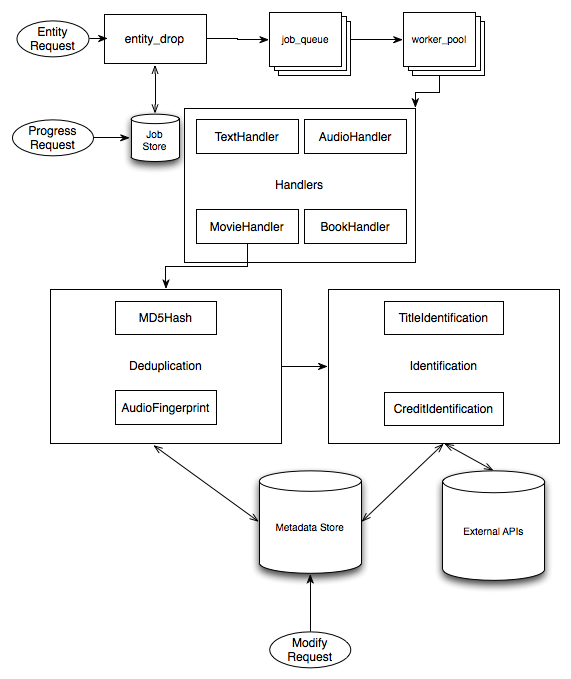
\includegraphics[scale=0.75]{system-overview.png}
\caption{The Librarian System Overview. Entity request start the flow through the system by 1. Creating a job for an entity. 2. Applying a handler for the entity. 3. Trying to identify the entity by deduplication or entity specific identifier method.}
\label{fig:system-overview}
\end{figure}


After deduplication or identification the job is linked to an item in the metadata store. The metadata store and job store are backed by a MongoDB database. This was chosen to allow the flexible schemas easily during development and direct storage or JSON objects obtained by external APIs. The job store can be queried with a job identification number for updates on the progress in the system or to place a modification request to manually update the metadata associated with an entity. \\

%------------------------------------------------

\subsection{Deduplication}
\label{sec:deduplication}
Deduplication is the first step in the ingestion process where the system looks for a match internally. Based on the entity type a variety of deduplication methods can be applied. Currently hashing and audio fingerprinting are used to resolve movie entities. These methods were picked for their computational efficiency and ability to identify duplicates without requiring exact matching (hashing vs. fingerprinting). \\

\subsubsection{Movie Entities}
\label{sec:dedup-movie-entities}
The deduplication process for movie entities consists of two steps. First a md5 hash is computed across the contents of the file and the metadata store is checked for any matches. This approach is brittle since the duplicate entities can still appear if two instances of the same film are added with different resolutions. A more flexible approach is to compute an audio fingerprint. We compute a fingerprint across a subsection of the file (first 10 minutes) since only a short duration is needed and the running time for computing a fingerprint across the entire file increases exponentially with file size. \\

Audio fingerprinting also has a large potential for identifying files, but requires extensive ground truth data and there are no open sources for such data. During the design stage we looked into fingerprinting movie trailers and checking increments of the films against these fingerprints. After some research however this method did not see either computationally efficient nor feasible since the fingerprint requires a minimum duration of approximately 10 seconds to effectively match an entity. \\


Although we were not able to use audio fingerprinting for identifying new files (because we lacked ground truth data), we were able to generate our own data and use that for deduplication purposes. We used the open source audio identification system called echoprint to generate audio fingerprints for every file. Echoprint generates unique audio fingerprints given an input audio file.  \\

The ffmpeg package was used for video file manipulation to ensure that each video was in the best format for fingerprint generation. As mentioned, we first cut each video to the first 10 minutes. We made the assumption that if 2 files have the same audio for the first 10 minutes, then they are actually the same entity. \\

After we generate our 10 minute video sample, we used ffmpeg to extract an audio file from the video. Echoprint was used on this to generate the unique audio fingerprint. These fingerprints were stored as part of our metadata and are used for deduplication.  \\


%------------------------------------------------

\subsection{Identification}
\label{sec:identification}
Unlike deduplication, identification is used to establish the identity of a file by looking at outside sources. These sources are assumed to have valid ground truth data by which some computation can be checked. For analysis purposes, all identification methods were when matching an entity, but in future iterations once identity is established the handler can return successfully. This allows the author of a handler to prioritize how different identification methods are run to optimize for precision or runtime. To establish the identity of movies two identifiers were used, title identifiers and credit identifiers. \\

\subsubsection{Title Identifiers}
\label{sec:title-identifier}

Title identification works in two steps. First, the title is cleaned by splitting the string on alphanumerics and removing stop words. Second, the cleaned title is checked against an internal database of known movie titles. An exact and a fuzzy match are performed. Possible matches are then queries against online sources (such as IMDB) to acquire metadata. \\

The title identification process was developed using the corpus of seed data. Using the filenames in the seed data a set of stop words was compiled eliminating many false positives. This method is computationally very inexpensive and has a high precision as \ref{sec:performance} shows. We also try to extract the year from the title string to find an exact match for film remakes. \\

Once the string is clean we use an internal database of film names to find potential matches to query against online sources. This is allows an arbitrary amount of fuzzy matching by querying the local database and avoids any rate limiting issues when making requests to online sources. This also allows us to match a cleaned string to a valid string since the local datastore was scraped from the same online sources that are queried. \\

\begin{figure}[H]
\center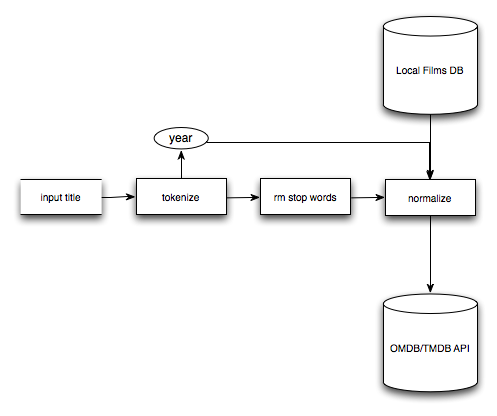
\includegraphics[scale=0.75]{title-identifier.png}
\caption{Netflix Home Screen. The first film display has the resume option (play icon overlay).}
\label{fig:title-identifier}
\end{figure}


\subsubsection{Credit Identifiers}
\label{sec:credit-identifier}

For many files in the initial corpus titles parsed successfully at a high rate since the data was relatively clean, however the method is very brittle and can easily deliver false positives if a file is slightly misnamed or comes from a dirty source. To match more effectively the credit identification method was implemented. This method performs optical character recognition (ORC) on the credits of a film and tries to extract actor names from the text. These names can then be queried against an online source and the intersection of the films the actors appear in can be used to establish identity. \\

This method proved to be the most computationally expensive and required heavy optimization to get an operational prototype implementation. The film is cut to contain only the last five minutes and then a frame is generated every three seconds. The raw text from each frame is then processed to heuristically clean it and reduce potential search tokens. The OCR, using the Tesseract library, can produce many false results which cause the runtime of the fuzzy searching to take on the order of minutes. To reduce this runtime tokens are eliminated by several heuristics such as length and removing excluded characters. The fuzzy searching queries an in-memory SQLite database of known actor names and uses the Python FuzzyWuzzy library to score matches. \\

Some optimizations for this fuzzy matching process were restricting the number of choices by finding the intersection of matches between first and last name instead of searching for a first name last name string together. Additionally, since the credit frames are ordered with the leading actors first, the OCR is performed in a streaming fashion since an intersection of a single film can likely be found within the first several frames which contains the leading actors. \\

The tokens extracted from the credit frames are queried against a local datastore of actor names for the same performance reasons as the title identifier. This ground truth data was scraped from the TMDB and OMDB apis and contains approximately 400,000 actor names. Moving the implementation to a compiled language may show better results since the performance costs will be lower and some of these optimization methods have the potential to miss potential matches if the heuristic is too strict. \\

\begin{figure}[H]
\center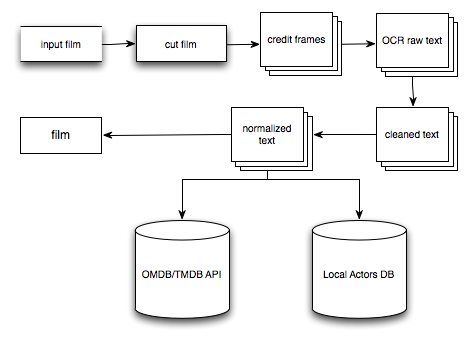
\includegraphics[scale=0.75]{credit-identifier.png}
\caption{Netflix Home Screen. The first film display has the resume option (play icon overlay).}
\label{fig:credit-identifier}
\end{figure}


\section{Performance}
\label{sec:performance}
%TODO

%------------------------------------------------

%------------------------------------------------
\subsection{Handlers}
\label{sec:handlers}
%TODO

%------------------------------------------------
\subsection{Identifiers}
\label{sec:identifiers}
%TODO

%------------------------------------------------


\section{Future Work}
\label{sec:future-work}

The librarian was designed to be easily extended. Just as we currently have Movie Handlers, the librarian can handle text files, audio files, and TV shows as well. \\

Although not currently part of the system, crowd sourcing would be very valuable in this kind of system. Having the ability for users to report mistakes would be great in cases where the librarian fails to correctly identify an entity. \\

Ideally the librarian would have the ability to manage the whole media server. On a very basic level that means having the ability to move files. We would extend that functionality to be able to specify some configuration file which would be able to specify different entity types and the correct way to categorize them. \\

We also plan to add a client that is able to interact with different sources of files and have the ability to prompt the librarian to handle new files. For example, having a torrent client that downloads files into the system and then have the librarian deal with deduping, identifying, and correctly indexing the file. \\

In addition to adding more features there is room for optimization. Given enough data on our identifiers, in the future we can prioritize them differently to obtain higher precision. \\

It's possible to move some of the code to a compiled language to improve performance, which would allow some of our heuristics (e.g: Credit Identifier) to not only take less time but also to have better accuracy. \\ 


%------------------------------------------------
\section{Conclusions}
\label{sec:conclusions}
%TODO

%------------------------------------------------


\end{document}